\section{E2 policy evidence}
\label{app:e2policy}
The E2 handoff is independently verified by
\path{tools/verify_portable_32_cpu.py}. Its package SHA256 is
\path{079e2b7e146b1706c2500ac9a3c4a5ff0c4310885cc013907e9b86c754399aa3};
the extracted package contains 32 cells, 36 attempts, 20 strict P1+ results,
12 scientific negative results, and four retained technical-invalid attempts.
No checkpoint was retrained or selected after physical execution. The all2
reference is one cell per window; each PPO cell is a repeated execution of the
same frozen checkpoint, not a new training seed.

\begin{table*}[t]
\centering
\small
\caption{Complete E2 policy summary. Costs are means over three PPO repeats or
the single all2 anchor in each window. A negative arm can have lower cost while
still violating the strict deadline contract.}
\label{tab:e2appendix}
\setlength{\tabcolsep}{5pt}
\par\vspace{4pt}
\begin{tabular*}{0.92\linewidth}{@{\extracolsep{\fill}}llrrrrr@{}}
\toprule
Arm & training environment & R P1+ & S P1+ & cost R & cost S & offline outcome\\
\midrule
all2 & anchor & 1/1 & 1/1 & 4.200 & 4.200 & 120/120\\
C-2 & C & 0/3 & 0/3 & 2.730 & 2.950 & 4--13 on time\\
C-1 & C & 3/3 & 3/3 & 2.357 & 2.449 & 120/120\\
C30-1 & C30 & 3/3 & 3/3 & 2.073 & 2.084 & 120/120\\
C30-2 & C30 & 3/3 & 3/3 & 2.051 & 2.103 & 120/120\\
C30-3 & C30 & 0/3 & 0/3 & 1.899 & 2.090 & 106--114/120\\
\bottomrule
\end{tabular*}
\end{table*}

The physical package stores both C and C30 predictions for each cell. Comparing
the frozen prediction labels with the final physical labels gives 32/32
feasibility-direction agreement for C and 20/32 for C30. Window-cost MAE is
0.0804 and 0.4657 scenario USD, respectively; these metrics use the same
registered observation-window ledger and do not estimate provider billing.
The C30 prediction marks C30-3 feasible in both windows, while all six
physical repeats fail the offline deadline. This is a false-positive deployment
case, not a reason to remove the negative cells.

The package also retains the exact attempt history, source and tensor hashes,
request terminals, controller events, lifecycle manifests, budget receipts, and
CPU recomputation for every cell. The four technical-invalid attempts remain in
the audit trail and are excluded from scientific repeat counts. The evidence is
bounded to two locked windows, two A100 GPUs, one Qwen model, five checkpoints,
and the declared synthetic-API scenario ledger.

\subsection{Frozen PPO training and selection contract}
\label{sec:ppo-training-contract}
The capacity policy uses a 30-dimensional observation, a shared MLP with
 two 256-unit ReLU layers, three capacity logits, and a scalar value head.
The four-logit offline head is masked to its sole legal action.
Training runs in CPU replay with guard disabled, using C or C30 and
2,100-step episodes and rollouts. Adam uses learning rate $3\times10^{-4}$
and numerical epsilon $10^{-5}$; PPO uses discount $0.9995$, GAE parameter
$0.999$, clip $0.2$, four update epochs, minibatches of 64, value coefficient
$0.5$, entropy coefficient $0.01$, and gradient norm limit $0.5$.
Advantages are normalized and value loss is clipped; the learning rate
is constant. These settings are recovered from the frozen configuration,
not retuned for the deployment results.

Training uses three development windows with prefix \texttt{train\_}
and suffix \texttt{\_v2} for the burst-offline, recovery, and steady regimes.
Selection uses the corresponding three \texttt{validation\_*\_v2} windows
with deterministic C30 replay, guard disabled, and P1+ required separately
in every window. Eligible checkpoints are ordered by equal-window mean
cost, checkpoint index, and seed. E2 reuses the two previously locked
Bridge recovery and steady inputs; these are distinct files from the
selection inputs. The training contract specifies paired seeds 101--105;
Table~\ref{tab:ppo-frozen-coordinates} gives the actual selected checkpoints.
The accompanying \texttt{PPO\_TRAINING\_CONTRACT.json} records the configuration,
selection-input hashes, and checkpoint identities.
Table~\ref{tab:ppo-frozen-coordinates} maps the paper labels to the archived
identifiers. In those identifiers, \texttt{r2} denotes the second eligible
checkpoint, \texttt{s101} the seed-101/episode-40 matched pair, and
\texttt{s103} the best eligible checkpoint within seed 103; the reference
is deployed as \texttt{ppo\_C30\_raw}.

\begin{table}[t]
\centering
\small
\caption{Paper labels and frozen checkpoint identities. Steps are those
reached by the selected checkpoint. C30-2 is the registered reference.}
\label{tab:ppo-frozen-coordinates}
\setlength{\tabcolsep}{2pt}
\par\vspace{4pt}
\begin{tabular*}{\linewidth}{@{\extracolsep{\fill}}llrrr@{}}
\toprule
Label & Archive ID & Seed & Episode & Steps\\
\midrule
C-1 & C-s101 & 101 & 40 & 84,000 \\
C-2 & C-r2 & 103 & 100 & 210,000 \\
C30-1 & C30-r2 & 101 & 25 & 52,500 \\
C30-2 & C30-ref & 101 & 40 & 84,000 \\
C30-3 & C30-s103 & 103 & 75 & 157,500 \\
\bottomrule
\end{tabular*}
\end{table}

\subsection{Retrospective E2 lifecycle diagnosis}
\label{sec:e2-lifecycle-diagnosis}
We diagnose all 32 accepted physical runs and their 24 frozen C/C30
predictions without retraining or selecting new checkpoints.
The two prediction configurations differ only in startup time
(69.219\,s versus 30\,s). Window launch-to-ready time exceeds 60\,s in
196 of 218 observed generations; the median of the 30 PPO runs' startup
medians is 87.92\,s. These are descriptive lifecycle measurements,
not independent experimental replicates.

C-2 exposes the interaction with the 60\,s cooldown, which starts at a
target change rather than at readiness. In the first recovery run, its
first window restart launches at 120.01\,s, becomes ready at 223.89\,s,
and enters draining at 224.01\,s without admitting work. The matched C
prediction becomes ready at 189.22\,s and drains at 190\,s, also without
admissions. C30 becomes ready at 150\,s; although the policy proposes zero
capacity, cooldown holds one GPU until 180\,s, admitting eight offline
requests. Across all six physical C-2 runs, 72 of 73 restarts longer than
60\,s enter draining within two seconds of readiness. All 687 offline
misses are already overdue before dispatch or remain undispatched at cutoff.

The other negative checkpoint has a milder queueing failure:
60 of C30-3's 65 offline misses are overdue before dispatch, while all
requests eventually complete. Long startup alone does not imply failure:
C-1 passes despite 78 of its 84 window restarts exceeding 60\,s,
retaining capacity to clear its queues. C30-1 and C30-2 also pass,
generally keeping a worker available after restarting.
These archived trajectories explain a concrete failure pathway and why
C detects its feasibility consequence. They do not establish a general
ranking of startup models or attribute every physical timing difference
to startup alone.


\begin{figure*}[t]
\centering
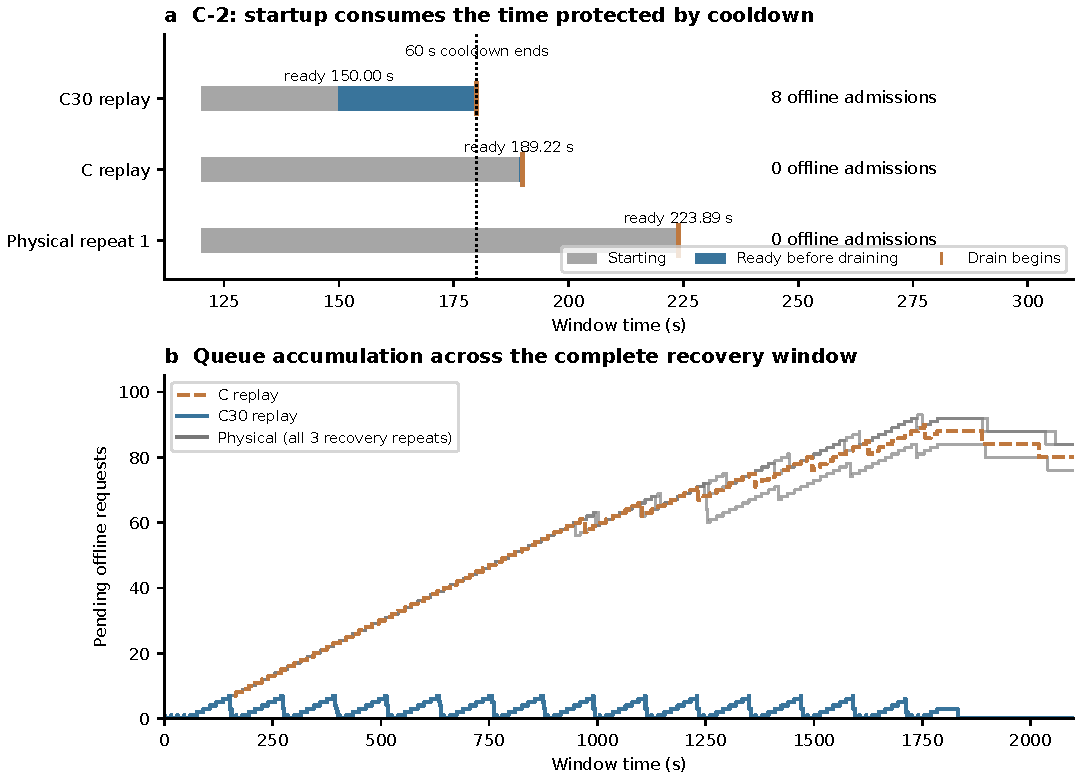
\includegraphics[width=\textwidth]{mechanism_diagnosis.pdf}
\caption{Retrospective C-2 recovery diagnosis. Top: the first window
restart of the first formal negative run and its frozen C/C30 predictions;
admissions count offline requests dispatched during that instance generation.
The dotted line marks cooldown expiry, measured from the target change.
Bottom: pending offline queues in both predictions and all three physical
recovery repeats. The text summarizes both windows and the passing-policy controls.
No new physical runs are introduced.}
\label{fig:e2-cooldown-diagnosis}
\end{figure*}
